% Original ArchDiagram Studio template. Edit labels and dimensions, not inferred facts.
\documentclass[tikz,border=10pt]{standalone}
\usepackage[T1]{fontenc}
\usepackage{lmodern,amsmath,amssymb}
\usetikzlibrary{arrows.meta,positioning,calc}
\definecolor{ink}{HTML}{202020}
\definecolor{blue}{HTML}{202020}
\definecolor{violet}{HTML}{202020}
\definecolor{teal}{HTML}{202020}
\tikzset{block/.style={draw=teal,fill=teal!4,rounded corners=4pt,minimum width=23mm,minimum height=12mm,align=center,inner sep=6pt},projection/.style={block,draw=violet,fill=violet!4},flow/.style={-{Latex[length=2mm]},draw=ink!75,line width=.8pt,rounded corners=3pt},note/.style={font=\small,text=ink!75,align=center}}
\begin{document}
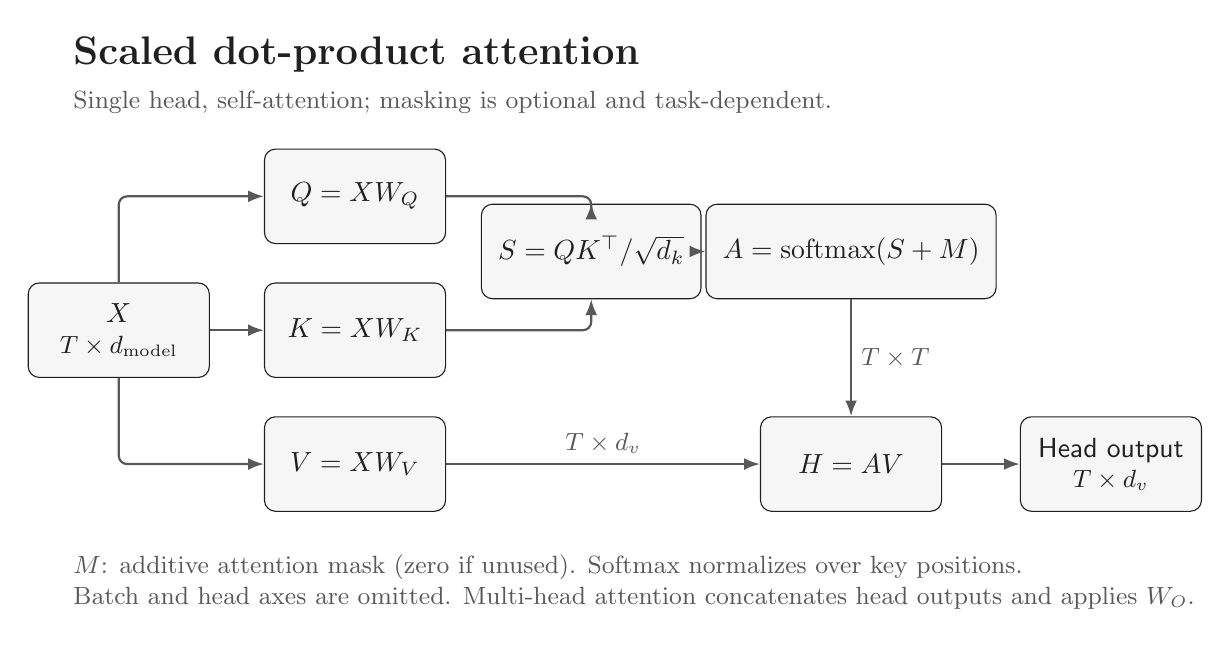
\begin{tikzpicture}[font=\sffamily,text=ink]
\node[anchor=west,font=\Large\bfseries] at (-.7,3.5) {Scaled dot-product attention};
\node[anchor=west,note] at (-.7,2.9) {Single head, self-attention; masking is optional and task-dependent.};
\node[block,draw=blue,fill=blue!4] (x) at (0,0) {$X$\\[-1pt]\small $T\times d_{\mathrm{model}}$};
\node[projection] (q) at (3,1.7) {$Q=XW_Q$};
\node[projection] (k) at (3,0) {$K=XW_K$};
\node[projection] (v) at (3,-1.7) {$V=XW_V$};
\node[block] (score) at (6,1) {$S=QK^\top/\sqrt{d_k}$};
\node[block] (softmax) at (9.3,1) {$A=\mathrm{softmax}(S+M)$};
\node[block] (weight) at (9.3,-1.7) {$H=AV$};
\node[block,draw=blue,fill=blue!4] (out) at (12.6,-1.7) {Head output\\[-1pt]\small $T\times d_v$};
\draw[flow] (x.north) |- (q.west);
\draw[flow] (x.east) -- (k.west);
\draw[flow] (x.south) |- (v.west);
\draw[flow] (q.east) -| (score.north);
\draw[flow] (k.east) -| (score.south);
\draw[flow] (score) -- (softmax);
\draw[flow] (softmax) -- node[right,note] {$T\times T$} (weight);
\draw[flow] (v) -- node[above,note] {$T\times d_v$} (weight);
\draw[flow] (weight) -- (out);
\node[note,anchor=west,align=left] at (-.7,-3.2) {$M$: additive attention mask (zero if unused). Softmax normalizes over key positions.\\Batch and head axes are omitted. Multi-head attention concatenates head outputs and applies $W_O$.};
\end{tikzpicture}
\end{document}
